\section{Dynamik}
\begin{minipage}{\linewidth} 
    \centering
%    \vspace{-2cm}
     \[ \texttt{Gelenkekräfte/Momente } Q
     \mathrel{\mathop{\rightleftarrows}^{\mathrm{Direkte Dynamik}}_{\mathrm{Inverse Dynamik}}}
      \texttt{Bewegung des Arbeitsgliedes } \ddot{q},\; \dot{q},\; q\]   
\end{minipage}

\begin{minipage}{\linewidth}
    \small 
    \begin{tabular}{p{3cm} p{2.7cm} p{3.2cm} p{3.2cm}}
        \hline
        \textbf{physikalische Grösse} & \textbf{generalisierten Beschreibung} &
        \textbf{Bezeichnung bei einem Schubgelenk}&
        \textbf{Bezeichnung bei einem Drehgelenk}\\ \hline
        generalisierte Koordinate & q &\textit{d} in [m]& $\theta$ in [rad]\\
        Masse, Trägheitsmoment & M & \textit{m} in [kg] & $J_L$ in [$kgm^2$]\\
        antreibende Kraft bzw. Moment & $\tau$ & \textit{F} in [N]& $M_{Gel}$ in [Nm]\\
        Verschiedene Kräfte/ Drehmomente & $b(q,\dot{q})$ & $\hat{F}_D \cdot \dot{d}+ m \cdot g \cdot \sin\beta $& $F_D \cdot \dot{\theta} + m \cdot g \cdot l_s \cdot \cos \theta$\\ 
        \hline  
    \end{tabular}
    \hspace{0.5cm}\begin{minipage}{4cm}
        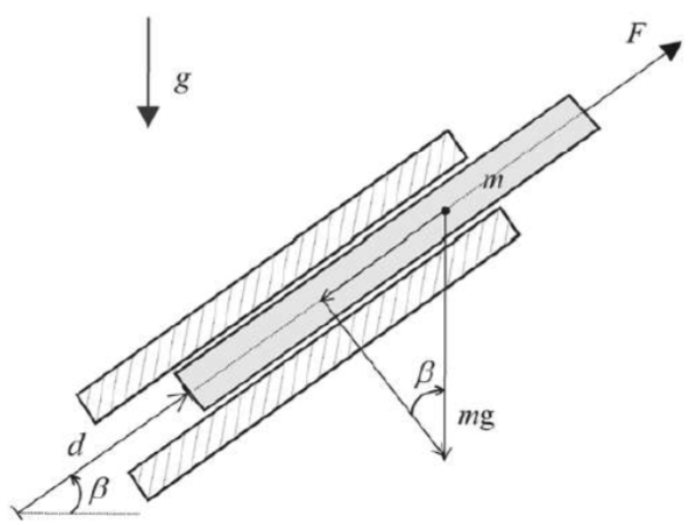
\includegraphics[width=0.9\linewidth]{./bilder/DynSchubgelenk.png}\newline
        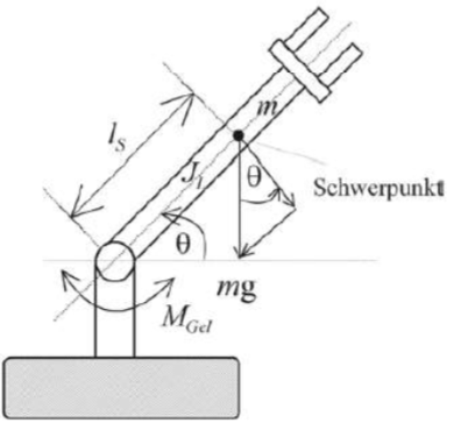
\includegraphics[width=0.8\linewidth]{./bilder/DynDrehgelenk.png}
    \end{minipage}
\end{minipage}
\begin{tabular}{p{4.5cm}lp{8.5cm}}
    \textbf{Dynamische Gleichung} \newline Roboter mit n Achsen&
    $Q = M(q)\cdot \ddot{q} + V(q,\dot{q})+ G(q)  $ &
    \small{
        Q: verallgemeinerte Kräfte (n\texttimes 1)\newline
        M: konfigurationsabhängige Massenmatrix (n\texttimes n)\newline
        V: Vektor nichtlinearer Term, der durch die Zentripetal- und die Coriolis-Beschleunigung entsteht (n\texttimes 1)\newline
        G: Vektor, der die Gravitationsterme enthält (n \texttimes 1)
    }\\
\end{tabular}

\subsection{Dynamik nach Lagrange}
\begin{tabular}{p{4cm}p{6cm}p{7.5cm}}
    \hline
    \textbf{Kinematische Energie eins Robotergiled i}&
    \[ \hspace{-0.5cm} E_{Kin, \; i} = \frac{1}{2} \cdot v_{Si}^T \cdot m_i \cdot v_{Si}+ \frac{1}{2} \cdot\omega_i^T  \cdot{}^0l_i  \cdot\omega_i \]
    \[ \hspace{-0.5cm} {}^0\dot{x}_{Si}=\begin{bmatrix}
    V_{Si}\\
    \omega_i
    \end{bmatrix}= {}^0 J_i \cdot \dot{q} \qquad{}^0J_i = \begin{bmatrix}
    J_{Ti}\\
    J_{Ri}
    \end{bmatrix} \]
&
   \small{
    $v_{Si}$: Geschwindigkeit des Schwerpunktes S vom Roboterglied i \newline
    $m_i$: Masse von Roboterglied i\newline
    ${}^0l_i$: Trägheitsmatrix von Roboterglied i (bezogen auf Schwerpunkt von i und ausgedrückt im Basiskordinatensystem \{0\}) \newline
    ${}^0J_i$: auf Roboterglied i bezogenen Jacobi-Matrix
    }\\\hline

    \textbf{Kinematische Energie aller Roboterglieder n}&
        \[ \hspace{-0.5cm} E_{Kin} = \frac{1}{2}\sum_{i=1}^{n}( v_{Si}^T \cdot m_i \cdot v_{Si}+ \cdot\omega_i^T  \cdot{}^0l_i  \cdot\omega_i )\]&\\ \hline
\end{tabular}
%\clearpage

\begin{minipage}{0.5\linewidth}
    \textbf{Kinetische Energie}\\
    \[ E_{Kin}= \frac{1}{2} \cdot \dot{q}^T \cdot M\cdot \dot{q}  \]
    mit der Roboterträgheitsmatrix:\newline
    \[ M = \sum_{i=1}^{n} ( J_{Ti}^T \cdot m_i \cdot J_{Ti} + J_{Ri}^T \cdot {}^0l_i \cdot J_{Ri}) \]
    \[ \hspace{-0.3cm}E_{Kin}= \frac{1}{2} \cdot \dot{q}^T \cdot \left[ \sum_{i=1}^{n} ( J_{Ti}^T \cdot m_i \cdot J_{Ti} + J_{Ri}^T \cdot {}^0l_i \cdot J_{Ri}) \right]\cdot \dot{q} \]
\end{minipage}
\begin{minipage}{0.5\linewidth}
    \textbf{Potentielle Energie}\\
    \[ E_{Pot}=-\sum_{i=1}^{n} m_i \cdot g^T \cdot r_{Si} \]
    g: Vektor der Gravitationsbeschleunigung\newline
    $r_{Si}$: Vektor der von der Referenzposition auf den Massenschwerpunkt von Glied i weist
    \vspace{1.8cm}
\end{minipage}
\clearpage

\begin{minipage}{\linewidth}
    \begin{minipage}{0.5\linewidth}
        \subsubsection{Lagrange Gleichung}
        \vspace{-0.5cm}
        \[ L=E_{Kin}-E_{Pot} \]
        \[ L= \frac{1}{2}\cdot \dot{q}^T \cdot M \cdot \dot{q} -(- \sum_{i=1}^{n}(m_i \cdot g^T \cdot r_{Si})) \]
    \end{minipage}
    \begin{minipage}{0.5\linewidth}
        \[ Q_j = \frac{\diff}{\diff t} \left(\frac{\partial L}{\partial \dot{q}_j} - \frac{\partial L}{\partial q_j}\right) \quad \texttt{mit}\quad j=1,2,\dots, n\]
        $Q_j$= verallgemeinerte Kräfte\newline
        $q_j$= verallgemeinerte Koordinaten
    \end{minipage}
\end{minipage}


\begin{minipage}{0.75\linewidth}
    \subsubsection{Bewegungsgleichung}
    \vspace{-0.5cm}
    \[\hspace{-0.5cm}\begin{pmatrix}
        \tau_1\\
        \tau_2
    \end{pmatrix}=
    \underbrace{
    \begin{bmatrix}
    b_{11}&b_{12}\\
    b_{21}&b_{22}
    \end{bmatrix}}_{\texttt{Beschleunigung}}
    \begin{pmatrix}
    \ddot{\theta}_1\\
    \ddot{\theta}_2
    \end{pmatrix}+
    \underbrace{
    \begin{bmatrix}
    0 &h_{1,22}\\
    h_{2,11}&0\\
    \end{bmatrix}}_{\texttt{Zentrifugal}}
    \begin{pmatrix}
    \dot{\theta}_1^2\\
    \dot{\theta}_2^2
    \end{pmatrix}+
    \underbrace{
    \begin{bmatrix}
    h_{1,12} & 0\\
    0&0\\
    \end{bmatrix}}_{\texttt{Coriolis}}
    \begin{pmatrix}
    \dot{\theta}_1 \dot{\theta}_2\\
    \dot{\theta}_2 \dot{\theta}_1
    \end{pmatrix} +
    \underbrace{
    \begin{pmatrix}
    g_1\\
    g_2\\
    \end{pmatrix}}_{\texttt{Gravitation}}
    \]
\end{minipage}
\begin{minipage}{0.25\linewidth}
    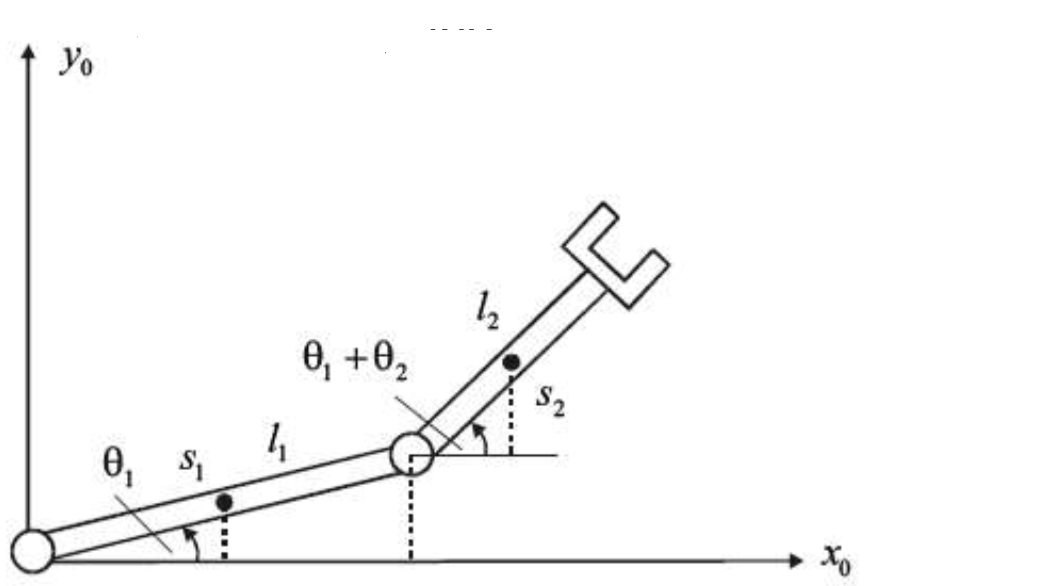
\includegraphics[width=\linewidth]{./bilder/PlanarRoboterBewegungsgleichung.png}
\end{minipage}

\begin{minipage}{0.7\linewidth}
    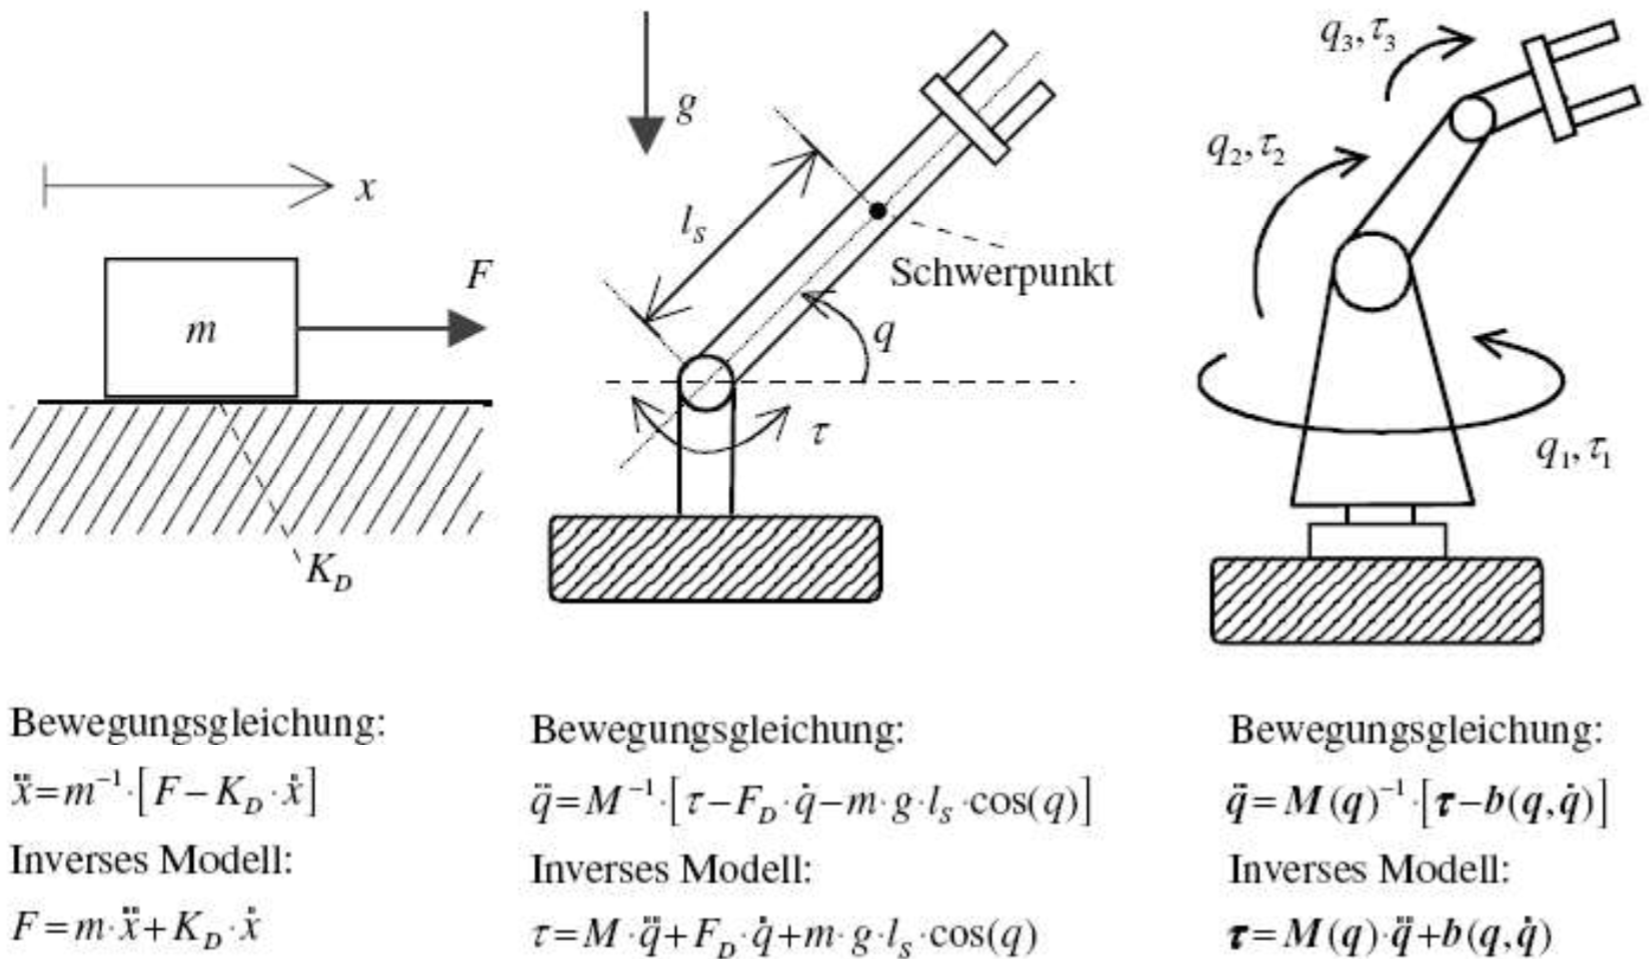
\includegraphics[width=\linewidth]{./bilder/DynMod.png}
\end{minipage}\\
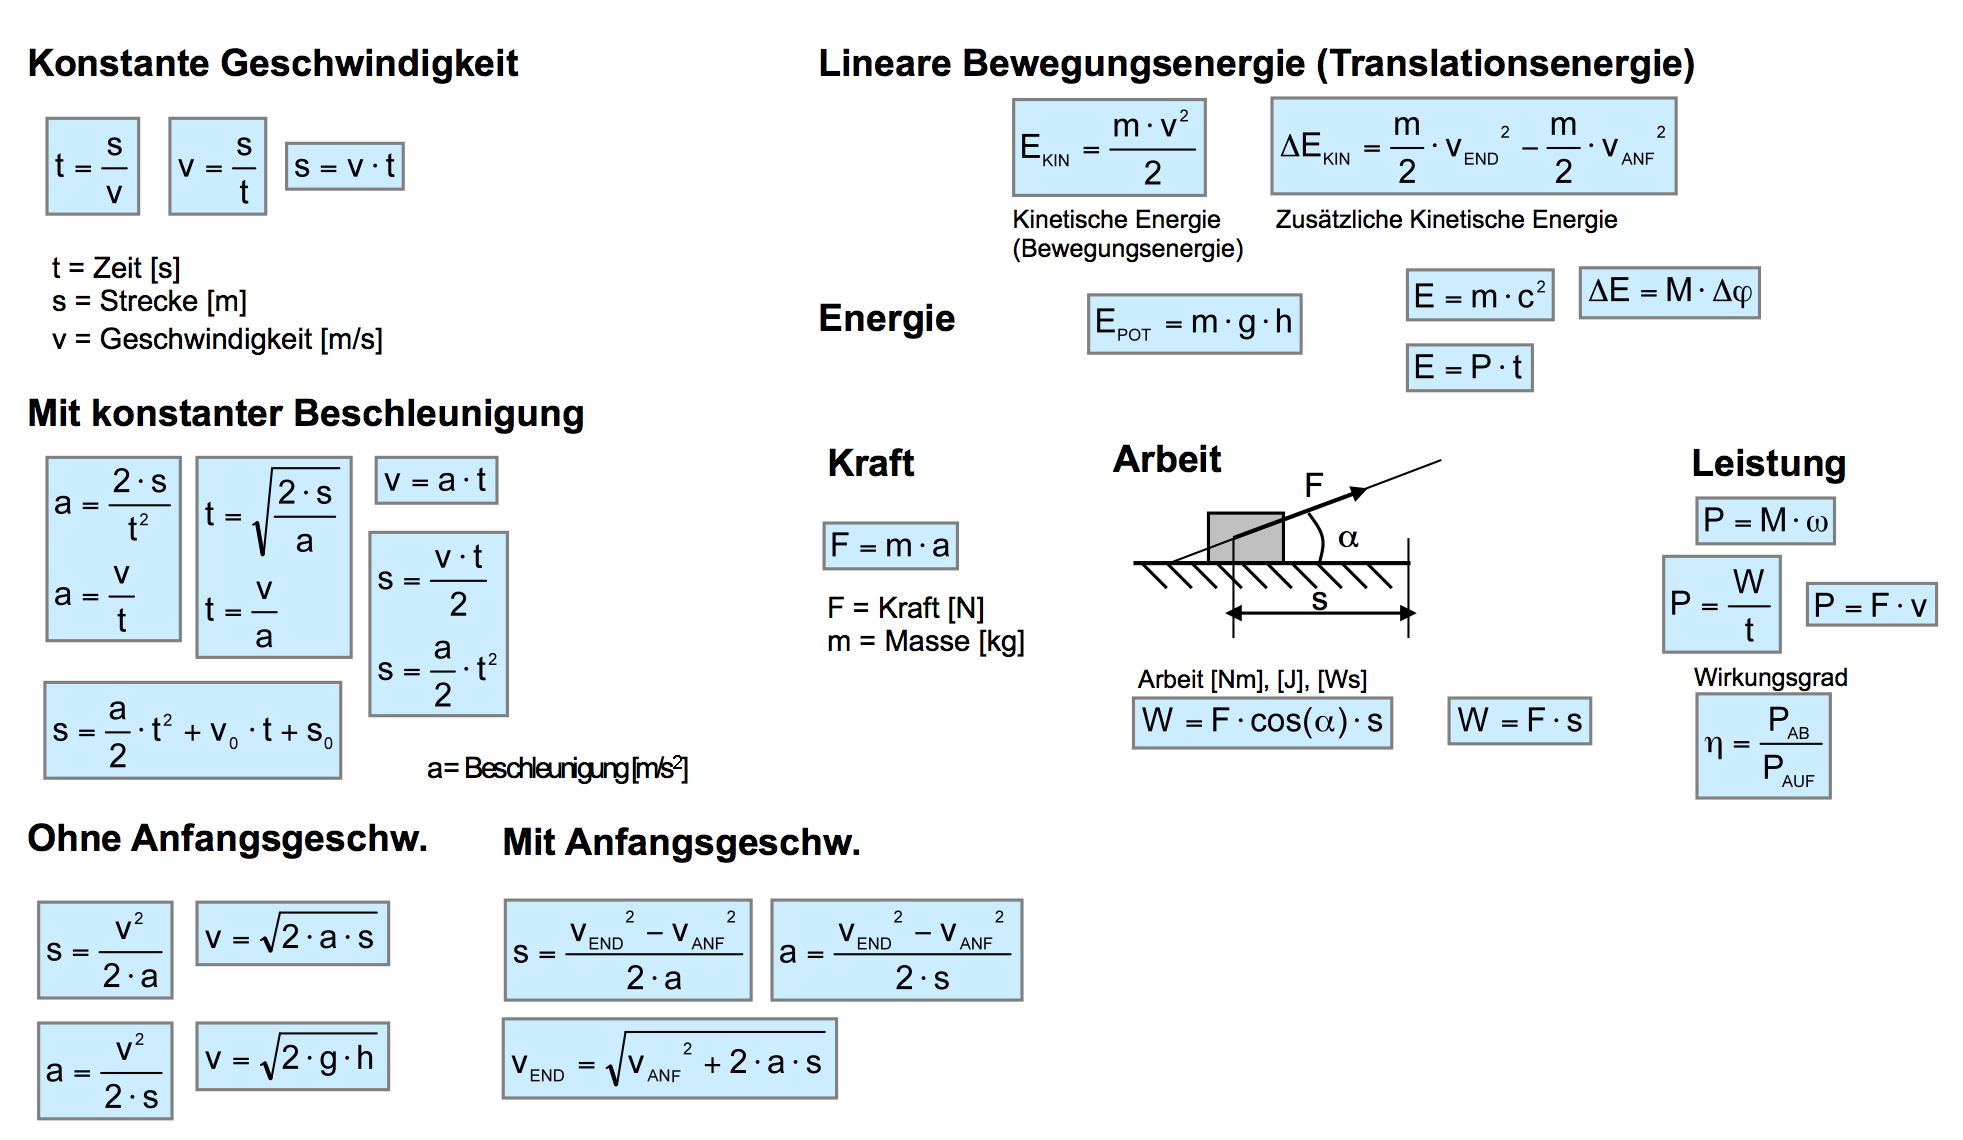
\includegraphics[width=17cm]{./bilder/kinematik.png}


